This section describes optimizations focused on reducing control flow and expanding block sizes which is necessary for high performance as seen in section~\ref{sec:lim_study}.

\subsection{Loop Unrolling}
As seen in Chapter~\ref{chp:streamit}, loop unrolling can be used to reduce the overhead of the loop header and to better expose Instruction Level Parallelism (ILP).
When dealing with tightly-knit loops, logical cores may perform poorly due to the fact that they execute many small blocks, thus increasing the Synchronization Cost and increasing the branch prediction requirements.
Unrolling loops will both reduce the number of blocks required to execute the loop and increase the size of the blocks, thus reducing the Synchronization Cost and increasing ILP.
For example, the innermost loop in Figure~\ref{lst:small} should be completely unrolled and its outer loop unrolled partially to increase the block size.
There are certain factors limit the usefulness of loop unrolling.
In the evaluated EDGE architecture, blocks may not have more than 32 load or store instructions.
This is due to the fact that block headers contain a 32 bit flag informing how many stores are in a block~\ref{putnam2010e2,smith2006edge}.
Therefore unrolling memory intensive loops will not necessarily increase the size of blocks drastically, however it will reduce the strain on branch prediction as it will generate multiple blocks with fixed branches.
Another issue is that unrolling loops with conditional statements may not help improve the size of the block as the conditional branches might still segment the new blocks.
So these loops should not be unrolled.

\begin{figure}[t]
\lstset{language=C,numbersep=4pt,basicstyle=\small,xleftmargin=.2\textwidth}
\begin{center}
\begin{lstlisting}

for(int i = 0; i < 1000; i++)
  for(int j = 0; j < 1000; j++)
     for(int k = 0;k < 5; k++)
         a[i][j] = a[i][j] * b[k][j];
\end{lstlisting}
\end{center}
\vspace{-1em}
\caption{Example of an inner-most loop which should be completely unrolled.}
\label{lst:small}
\end{figure}

\begin{figure}[t]
\lstset{language=C,numbersep=4pt,basicstyle=\small,xleftmargin=.2\textwidth}
\begin{center}
\begin{lstlisting}

for(int i = 0; i < 1000; i++)
  for(int j = 0; j < 1000; j++)
      a[i][j] = a[i][j-1] * b[i][j];
\end{lstlisting}
\end{center}
\vspace{-1em}
\caption{Example of a data dependency which can be removed by interchanging the loops.}
\label{lst:dep}
\vspace{1em}
\end{figure}


\subsection{Loop Interchange}
When dealing with nested loops there is one reason for interchanging the loops.
The case arises when interchanging the loop removes dependencies in the inner-most loop.
The dependency in Figure~\ref{lst:dep} can be removed by interchanging the loops. 
This allows us to unroll the inner loop efficiently, but also remove any kind of dependency between blocks.
Since two blocks from the same loop may execute on different cores, reducing any kind of data dependency is important as to minimize core communication.

\begin{figure}[t]
     \centering
     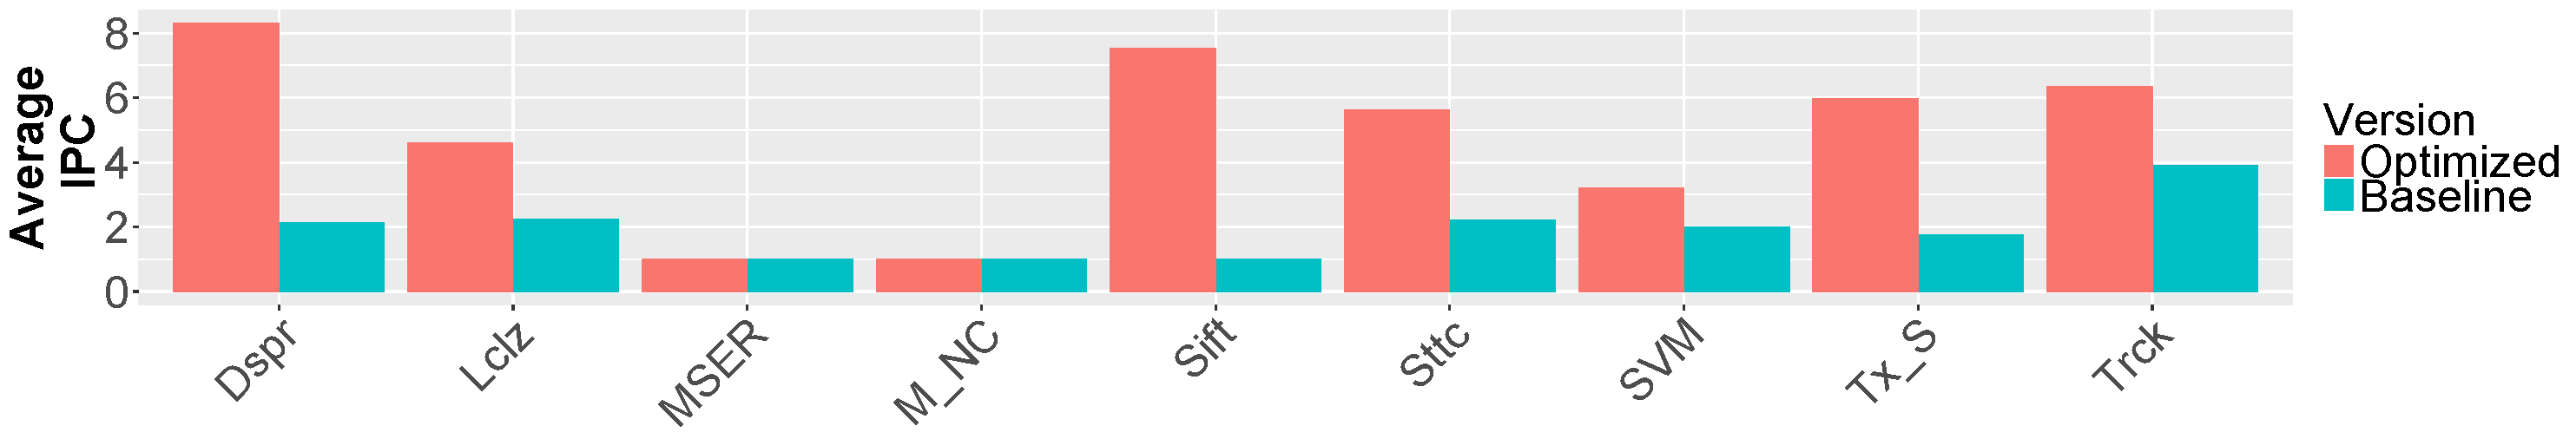
\includegraphics[width=\textwidth]{cases-paper/graphics/Exploration/ipc_comp.pdf}
\vspace*{-8mm}
     \caption{Average IPC using the optimal sized logical-core, with and without optimizations. Higher is better.}
     \label{fig:ipccom}
     \vspace{0.5em}
\vspace{5mm}
    \centering
    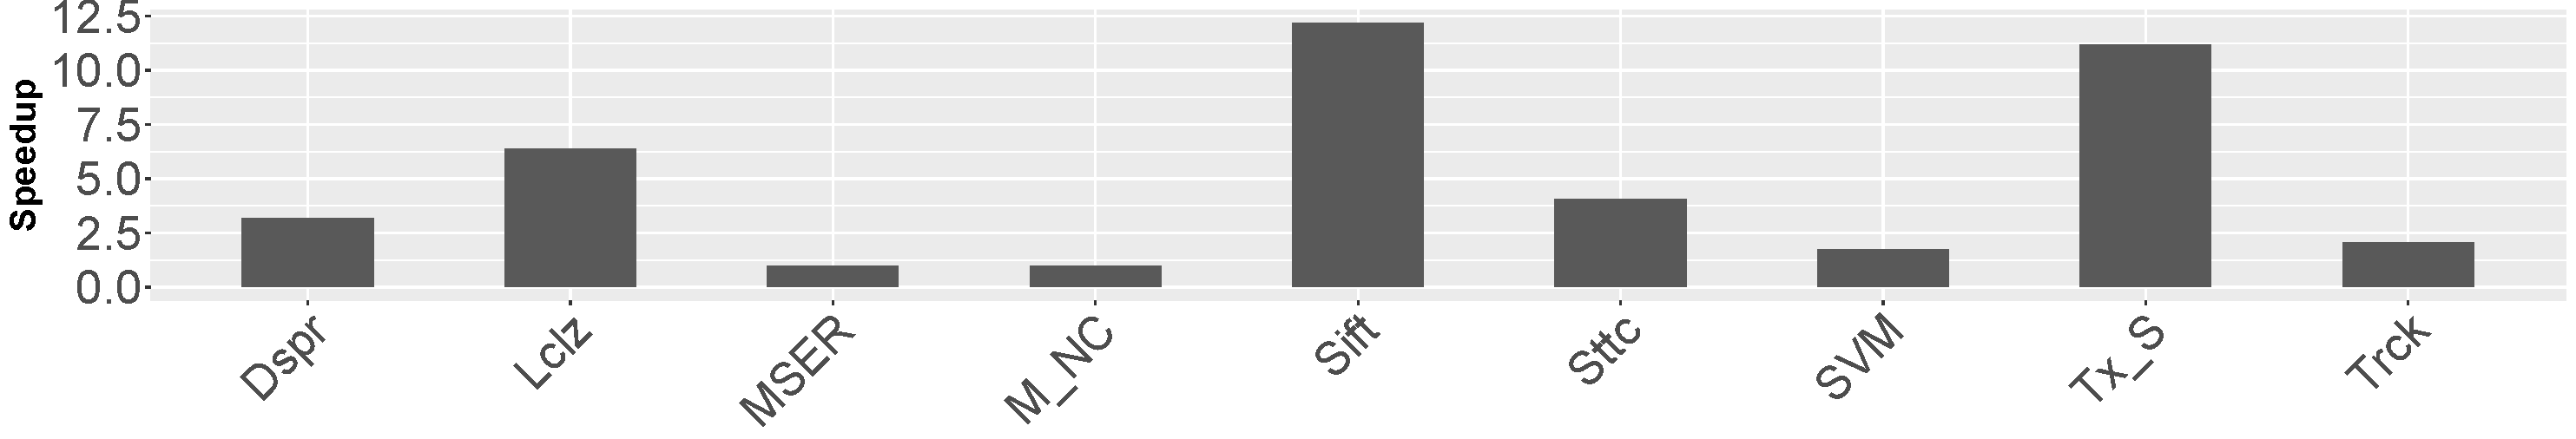
\includegraphics[width=\textwidth]{cases-paper/graphics/Exploration/comp_speed.pdf}
\vspace*{-8mm}
    \caption{Speedup from using code-optimizations over baseline source code using the same optimal sized logical-core.}
    \label{fig:speedcomp}
\vspace{5mm}
\end{figure}

\subsection{Predication and Hyperblock Formation}
EDGE compilers must split blocks whenever control-flow is present~\cite{smith2006edge}.
If a loop contains a conditional statement, the loop body has to be split in two unless if-conversion is applied.
Hyperblock formation aims to reduce branching and increase block size by combining two or more blocks into a single predicated block~\cite{smith2006edge}.
Hyperblocks reduce both synchronization cost and branch prediction requirements as discussed previously.
This is especially important in control-flow intensive loops where unrolling increases the number of conditional statements.

\vspace{5mm}
\subsection{Results}

While the optimizations described above and their tuning would be easy to implement in a compiler, this thesis did not have access to the compiler's source code.
Therefore the source code of the benchmarks is modified by manually interchanging or unrolling loops.
In the case of predication and hyperblock formation, simple if-then-else statements are converted into ternary operators whenever possible.
Statements are also re-ordered within the body of a loop to avoid having control flow in the middle of the body.
The source code modifications are then verified to have the intended effect by dissembling the binary produced by the compiler.
On average there are between 0 and 12 loops modifications depending on the benchmark.

The best static core fusion using the optimized code is compared with the unmodified code, both version compiled with \texttt{-O2}.
Figure~\ref{fig:ipccom} shows the resulting IPC for the baseline case and the optimized benchmarks when run on a core with the optimal number of fused core to maximize performance.
The IPC of the baseline is very low for the majority of the benchmarks which might give the impression that core fusion is rather inefficient.
However, after applying the simple optimizations described above, the average IPC is significantly increased in many cases.

Since optimizations change the total number of instructions, the actual speedup obtained using cycle count is also shown in Figure~\ref{fig:speedcomp}.
As can be seen, benchmarks \bm{MSER} and \bm{Multi-NCut} do not perform any differently.
This is due to the fact that none of these optimizations can be successfully applied on these benchmarks.
For the other benchmarks there is a significant improvements of up to 12$\times$ for \bm{Sift} when the optimizations are applied.
It is important to note that, whilst often the increase in IPC correlates with the speedup, this is not always the case.
In these situations, this is due to the fact that some of the optimisations also reduced the amount of computation required to complete the program; this is the case for \bm{Localization} and \bm{Sift}.

\paragraph{Summary}

Overall, this section shows that classical loop transformations can have a large impact on the performance of fused cores.
Without these optimizations, it would be more difficult to motivate the use of core fusion even at a static-level as the IPC does not deviate enough from a single core.
